\documentclass[final, hyperref, table]{beamer}
\mode<presentation>


 %\usepackage[english]{babel} % "babel.sty"
% \usepackage{french}                  % "french.sty"
%  \usepackage{franglais}               % "franglais.sty" (a defaut)
  \usepackage{times}            % ajout times le 30 mai 2003
 
%% --------------------------------------------------------------
%% CODAGE DE POLICES ?
%% Si votre moteur Latex est francise, il est conseille
%% d'utiliser le codage de police T1 pour faciliter la césure,
%% si vous disposez de ces polices (DC/EC)
\usepackage[utf8]{inputenc}
\usepackage[T1]{fontenc}


%% ==============================================================
%\usepackage{graphicx}
\usepackage{amsmath,amsfonts}
%\usepackage[table]{xcolor}
\usepackage{subfigure}
\usepackage{fancybox}
\usepackage{multicol}
\usepackage{wrapfig}
\usepackage{listings}
\usepackage{xcolor}

%\usetheme{Warsaw}
\usetheme{Frankfurt}
%\usetheme{JuanLesPins}
\setbeamercovered{transparent}


% telemeta red
\definecolor{telemetaRed}{rgb}{0.41568, 0.01176, 0.02745}   % #6A0307
\usecolortheme[rgb={0.41568, 0.01176, 0.02745}]{structure} 

\hypersetup{colorlinks, urlcolor=blue, linkcolor=}
% Display a grid to help align images
%\beamertemplategridbackground[1cm]

%We will get the normal bibliography style (number or text instead of icon) by including the following code
\setbeamertemplate{bibliography item}[text]
\setbeamerfont{caption}{size=\footnotesize}
% listings settings
\definecolor{lstComments}{rgb}{0,0.6,0}
\definecolor{lstBkgrd}{rgb}{1,1,0.8}
\definecolor{rouge}{rgb}{1.0,0,0}
\newcommand{\chref}[2]{
    \href{#1}{\color{rouge}\underline{#2}}
}
\newcommand{\dchref}[1]{
    \href{#1}{\color{rouge}\underline{#1}}
}
\newcommand{\curl}[1]{
    \color{rouge}\underline{\url{#1}}
}

\lstset{%
  language=Python, % the language of the code
  frame=single,  % adds a frame around the code
  commentstyle=\color{lstComments},% comment style
  backgroundcolor=\color{lstBkgrd},   % choose the background color
  basicstyle=\scriptsize,       % the size of the fonts that are used for the code
  keywordstyle=\color{blue},      % keyword style
  showstringspaces=false,          % underline spaces within strings only
}
\title[]{Web analysis tools for ethnomusicology}%\raisebox{2\height}{\includegraphics[width=0.4\textwidth]{img/logo_telemeta_1-1.pdf}}

\author[Guillaume et al.]{\small Guillaume Pellerin\inst{1}, Thomas Fillon\inst{1}, Joséphine Simonnot\inst{2}}


\institute[Parisson]{\scriptsize
  \inst{1}%
  Parisson, Paris, France\\
  \inst{2}%
  CREM, LESC, UMR CNRS 7186, MAE, Université Paris Ouest Nanterre La Défense, Nanterre, France\\
  
 {\tiny \textcolor{red}{\emph{This work was partially done inside the DIADEMS project\\ funded by the French National Research Agency ANR (CONTINT)}}}

 
\includegraphics[width=.3\linewidth]{img/parisson_logo_4_black_72_600px.png}
 \hfill
 \raisebox{-2ex}{
\includegraphics[width=0.1\linewidth]{img/logo_CREM.png}}}

\date{FMA 2015 Workshop, Paris}


\newcommand{\CREM}{Research Center for Ethnomusicology}
\setbeamertemplate{section page}
{
    \begin{centering}
    \begin{beamercolorbox}[sep=12pt,center,rounded=true, shadow=true]{part title}
    \usebeamerfont{section title}\insertsection\par
    \end{beamercolorbox}
    \end{centering}
\tableofcontents[currentsection, hideothersubsections]
}
\AtBeginSection[]{\frame{\sectionpage}}
% \AtBeginSection[] % Do nothing for \section*
% {
% \begin{frame}
% \frametitle{Outline}
% \tableofcontents[currentsection]
% \end{frame}
% }
\begin{document}%\footnotesize
\begin{frame}[plain]
  \begin{center}
    \raisebox{-1cm}{\includegraphics[width=0.4\textwidth]{img/logo_telemeta_1-1.pdf}}
  \end{center}
  \maketitle
\end{frame}

% \begin{frame}\frametitle{Outline}
%   \tableofcontents[hideallsubsections]
% \end{frame}


\section{Introduction}

\begin{frame}\frametitle{Introduction}
 \begin{block}{Context}
   \begin{itemize}
    \item \alert{Digital age}: Archiving and accessing tons of research data
    \item \alert{Network age}: Internet, social networks, mutualization of resources
    \item \alert{Open Access to knowledge and technoogies}: languages, formats, standards, licenses, open source
   \end{itemize}
\end{block}

\begin{block}{Challenges}
   \begin{itemize}
    \item \alert{musicologists} need music, metadata and search engines
    \item \alert{computer scientists} need music and semantic datasets
    \item both communities need to learn from one another to jointly develop tools for \alert{computational ethnomusicology}
    \item How do we \alert{grow and scale} data and technologies in a \alert{sustainable way}?
   \end{itemize}
\end{block}

%    \item Since 2007, the Research Center for Ethnomusicology (CREM) and Parisson
%      have been developing an innovative, collaborative and
%      open-source \alert{web-based multimedia platform} for \alert{humanities and social sciences research}.
   % \item Main goals:
   %   \begin{itemize}\scriptsize
   %     \setbeamertemplate{itemize subitem}[triangle]
   %   \item Preserve and easily access, visualize and annotate sound
   %     archives materials and metadata
   %   \item Fit the professional requirements from both sound
   %     archivists and researchers in ethnomusicology.
   %   \end{itemize} 

%    \item Official platform online since 2010 : 
%      \vspace{-0.1cm}\begin{center}
% \emph{Sound archives of the CNRS - Musée de l'Homme}
%        \colorbox{yellow!40} {\bf \url{http://archives.crem-cnrs.fr}}
%      \end{center}
%    \item This \alert{collaborative} platform support numerous aspects of the field of
%      \alert{ethnomusicology}, ranging from musical analysis to comparative
%      history and the anthropology of music. The platform also provides
%      many useful resources for the fields of anthropology, linguistics
%      and acoustics.
%    \end{itemize}

\end{frame}



\section[Telemeta]{The Telemeta platform}\label{sec:Telemeta}

\begin{frame}
  \frametitle{The Telemeta platform}
  \begin{block}{Open audio platform with metadata}
      \begin{itemize}
      \item \alert{access, preserve} and \alert{share} sound items
      \item enrich associated \alert{metadata} that
        contains key information on the context and significance of
        the recording.
      \item Telemeta = music + metadata + web
      \end{itemize}
    
  \end{block}
  \begin{block}{An open-source software}
    \begin{itemize}
    \item Telemeta, is a \alert{free and open source software} (\emph{GPL-like} licence)
       in accordance with \alert{open web standards}.
    \end{itemize}
    \vspace{-0.5cm}
    \begin{center}
      \raisebox{-0.4\height}{\includegraphics[width=0.3\textwidth]{img/logo_telemeta_800.png}}
\hspace{1cm}
      \colorbox{yellow!40}{\textbf{\url{http://telemeta.org/}}}
    \end{center}
  \end{block}
\end{frame}

\subsection{Features}
\begin{frame}[label=telemeta_features]{Telemeta features}
  \begin{block}{}
    \begin{itemize}
      \item \alert{Pure HTML5} web user interface including dynamic forms.
      \item \alert{On-the-fly audio analyzing}, transcoding and metadata
        embedding in various multimedia formats, provided through \emph{TimeSide}.
      \item \alert{Social editing} with semantic ontologies, smart workflows, human or automatic annotations and segmentations.
      \item \alert{User management} with individual desk, playlists, profiles
        and group access rights.
      \item \alert{High level search engine} (text, dates, locations, instruments, ethnic groups, etc...).
      \item \hyperlink{telemeta_languages}{\alert{Multi-language support} support (currently english, german, french, chinese, arabic and portuguese).}
      \end{itemize}
    \end{block}
\end{frame}


\subsection{Metadata}\label{sec:metadata}
\begin{frame}\frametitle{Metadata}
  \begin{block}{}
    \begin{itemize}
    \item Everything describing the context of a music record
    \item Valuable informations about the \alert{source of the data} and to the related \alert{work of
        peer researchers}.
    \item \alert{Collaborative editing} of metadata optimizes the continuous process of knowledge gathering
      and the \alert{enrichment} of the materials in the database.
    \item \alert{Standardization} of audio and metadata formats of long-term preservation
    \item \alert{Easy harvesting} with metadata standards protocols like
      \emph{Dublin Core} and \emph{OAI-PMH} (Open Archives Initiative
      Protocol for Metadata Harvesting).
    \end{itemize}
  \end{block}
% The metadata includes two different kinds of information about the audio item:
% \begin{itemize}
% \item contextual information and
% \item Descriptive and analytical information of the audio content
% \end{itemize}
\end{frame}


\begin{frame}[label=telemeta_metadata]{Ethnomusicological metadata}
\begin{block}{Contextual information}
  \begin{itemize}
  \item Geographic information
  \item Cultural information (population, related cultural elements, etc)
  \item Musical information (title, instruments, etc)
  \item Technical information (recording technical data, depositor, collector, year of the recording, year of publication of papers describing the work, etc)
  \end{itemize}
\end{block}

\begin{block}{Additional materials}
  \begin{itemize}
  \item iconographies (digitalized pictures, scans of booklets and
    field notes, and so on),
  \item hyperlinks
  \item biographical information about the collector.
  \end{itemize}
\end{block}

\end{frame}


% \begin{frame}{Metadata}{Descriptive and analytical information on the audio content}
% The second type of metadata consists of information about the \alert{audio content} itself. This metadata can provide information about the global content of the audio item or provide \alert{temporally-indexed information}. 
% Such information can be produced eithe
% r:
% \begin{itemize}
% \item by a human expert or
% \item by an automatic computational audio analysis.
% \end{itemize}
% And it can consist either in:
% \begin{itemize}
% \item Visual representation and segmentation or
% \item Annotations
% \end{itemize}

\subsection{Architecture}
\begin{frame}\frametitle{Telemeta architecture}
  \begin{center}
    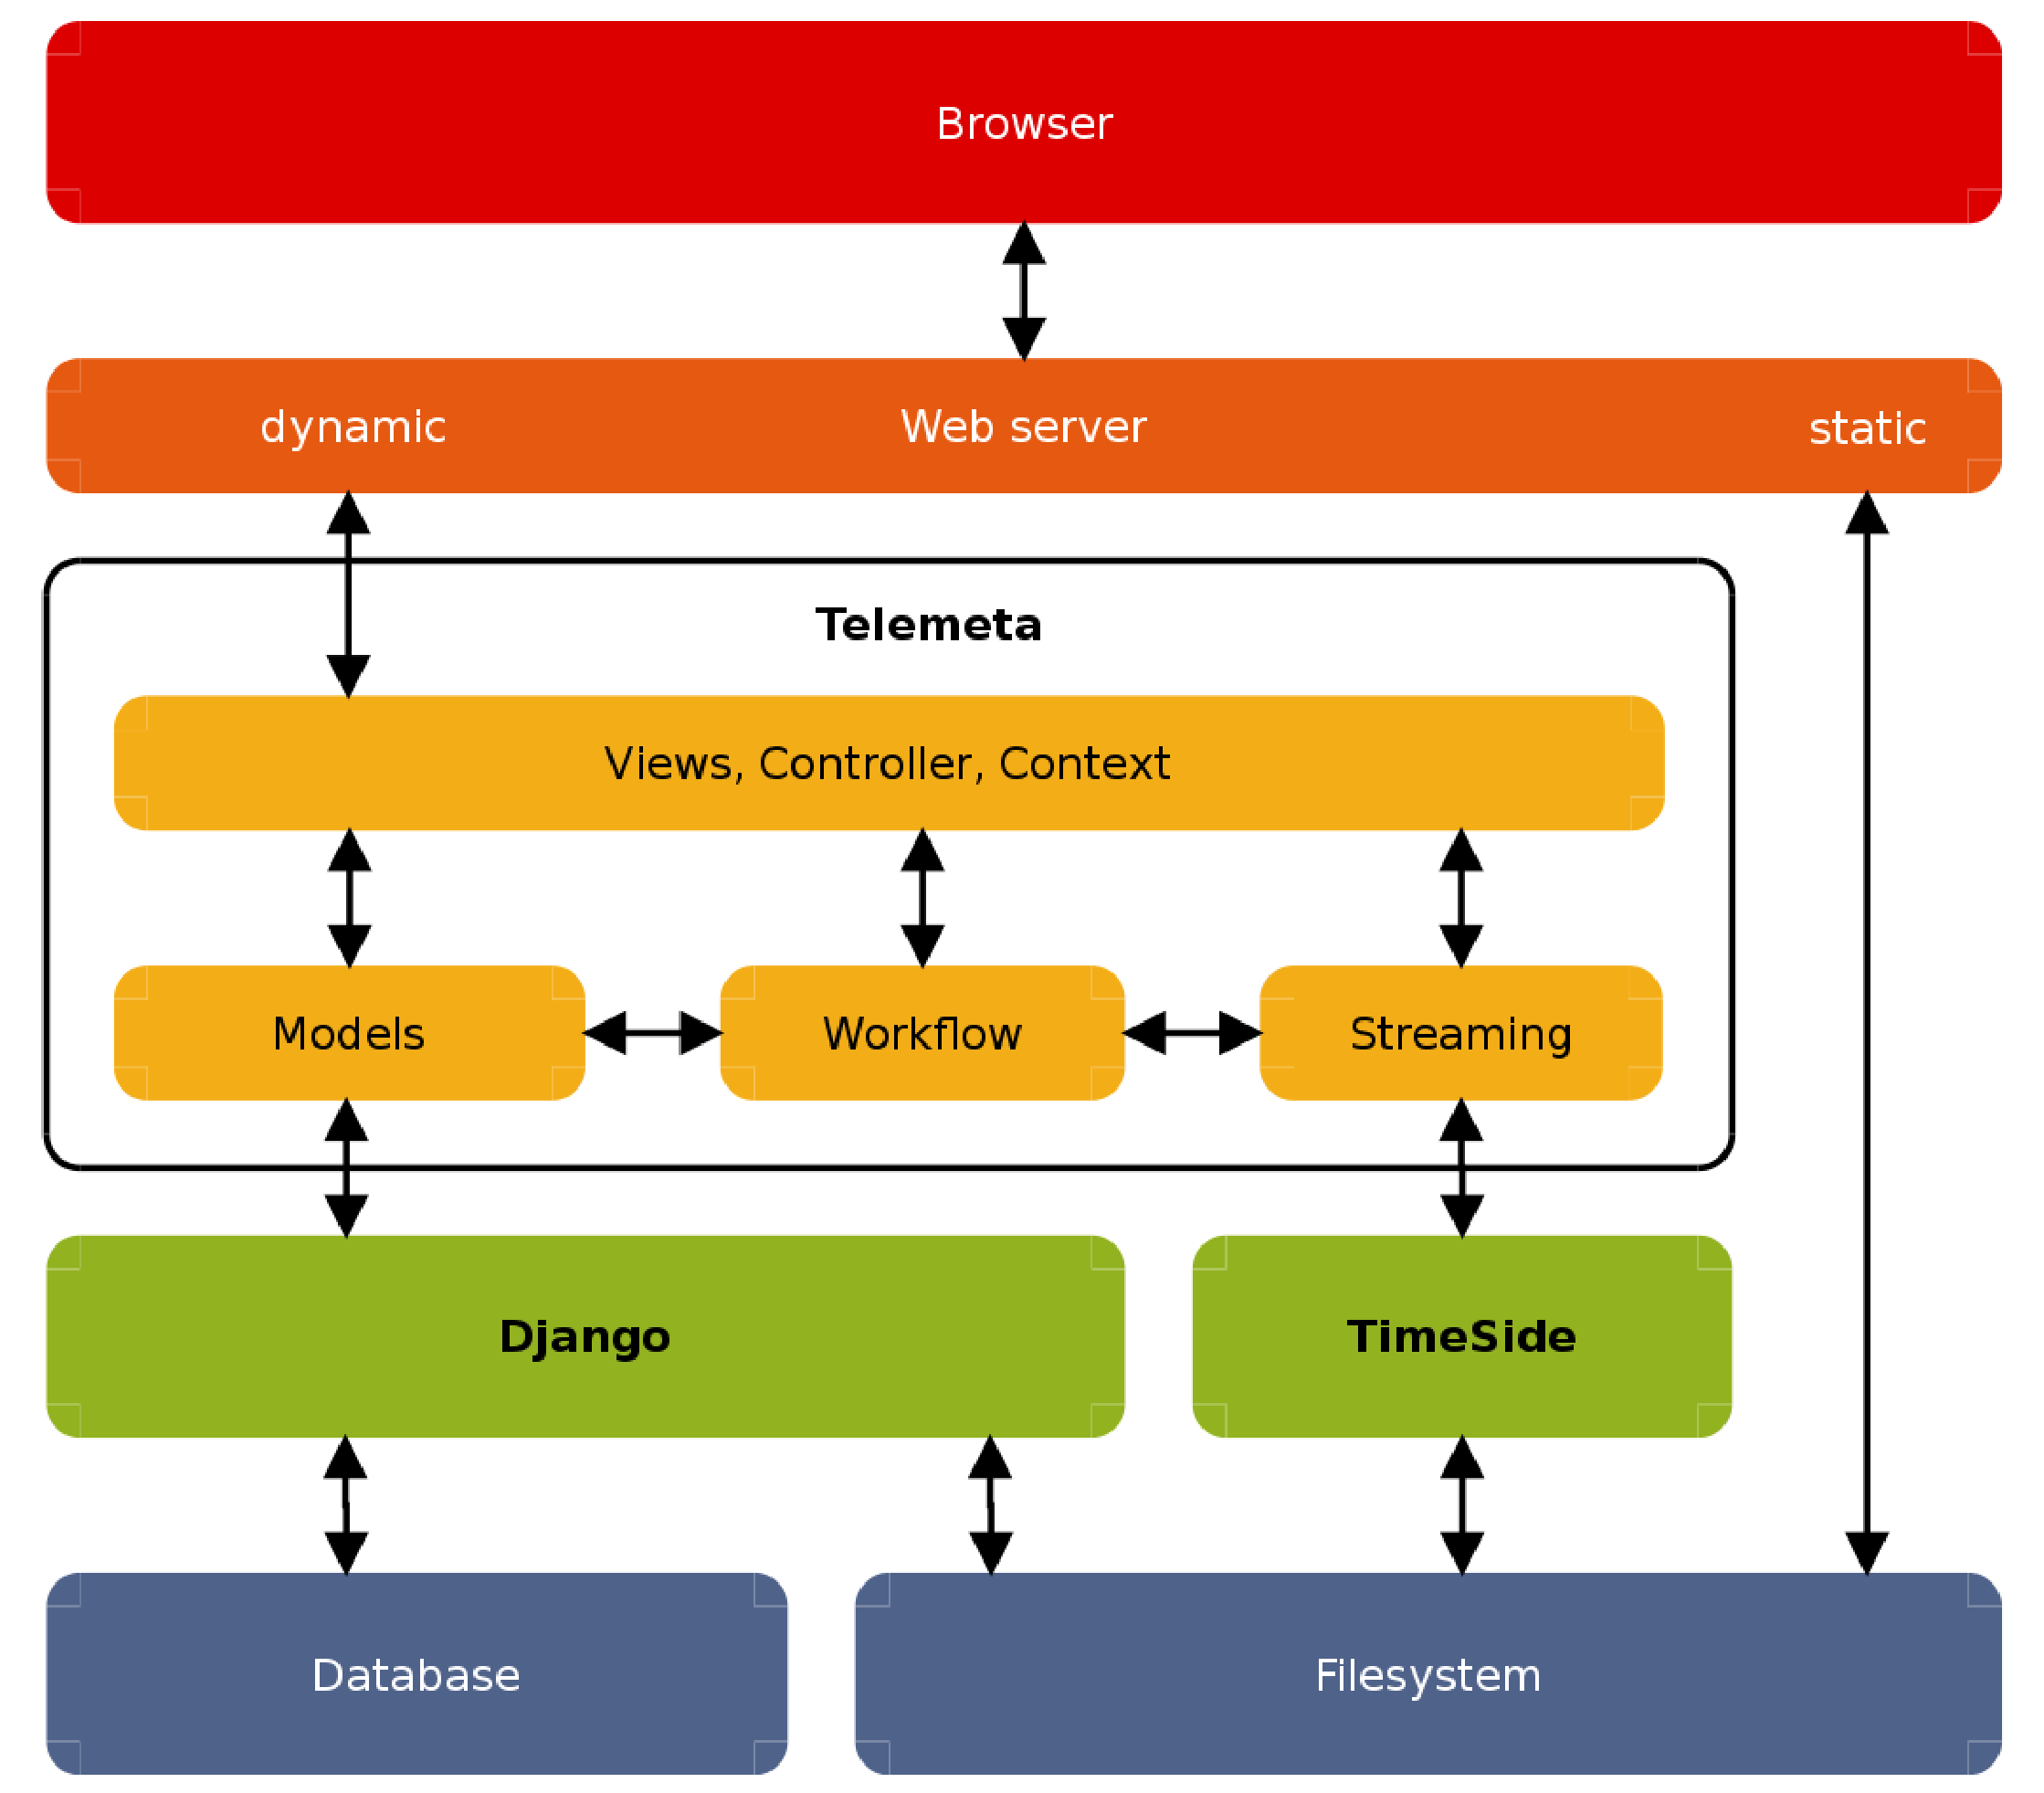
\includegraphics[width=0.75\textwidth]{img/TM_arch.pdf}
  \end{center}
\end{frame}


\begin{frame}[plain]{Telemeta UI (demo)}
  \begin{center}
    \fbox{\includegraphics[width=\linewidth]{img/telemeta_screenshot_en_2.png}}
  \end{center}

\end{frame}

  
% \end{frame}
\begin{frame}{Descriptive and analytical information}
{Visual representation and segmentation}
\scriptsize
\begin{columns}[T]
    \begin{column}{0.6\textwidth}
      \begin{block}{Visual representation of the sound}
       The embedded \alert{TimeSide} audio player allows for a selection
        of various visual representations of the sound (e.g. \alert{waveforms
        and spectrograms}) and some representations of computational
        \alert{analysis}.
      \end{block}
    \end{column}
    \begin{column}{0.3\textwidth}
      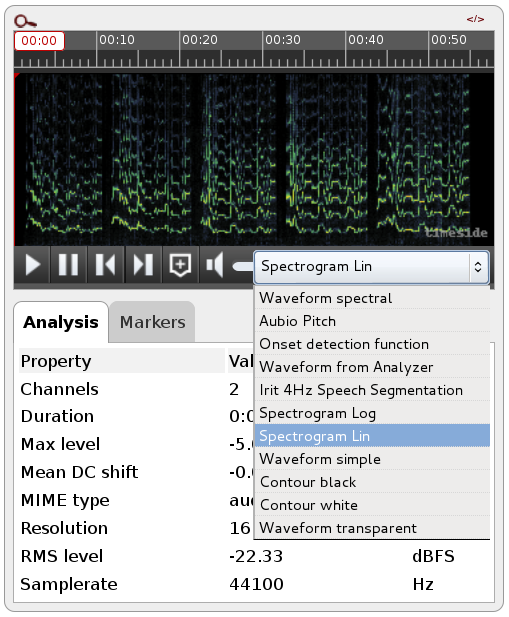
\includegraphics[width=\linewidth]{img/sound_representation.png}
    \end{column}
  \end{columns}
\vspace{-1.5cm}
  \begin{columns}[T]
    \begin{column}{0.6\textwidth}
   \begin{block}<2>{Segmentation}
        Automatic analysis can produce a list of \alert{time-segments}
        associated with \alert{labels} (e.g. detection of spoken versus
        singing voices, chorus, musical instrument categories, and so
        on).
\end{block}
    \end{column}
    \begin{column}{0.3\textwidth} 
  %Detection of spoken voices in a song
    \end{column}
  \end{columns}
  \begin{center}
    \includegraphics<2>[width=0.65\linewidth]{img/IRIT_Speech4Hz.png}
  \end{center}

  
\end{frame}
\begin{frame}{Descriptive and analytical information on the audio content}{Annotations}%\scriptsize
  \begin{columns}[T]
    \begin{column}{0.6\textwidth}
      \begin{block}{Markers}%\tiny
        \begin{itemize}
        \item The embedded audio player also enables annotation of the
          audio content through \alert{time-coded markers}.
        \item These annotations are \alert{indexed through the database}.

        \item Users can create their own annotations and \alert{share} them with colleagues.
   
          % \item \emph{The possibility for experts to annotate
          %   time-segments
          %   over a zoomable representation of the sound is currently
          %   under development in order to improve the accuracy and
          %   the
          %   quality of time-segment-based annotations.}
        \end{itemize}

      \end{block}
    \end{column}

    \begin{column}{0.4\textwidth}
      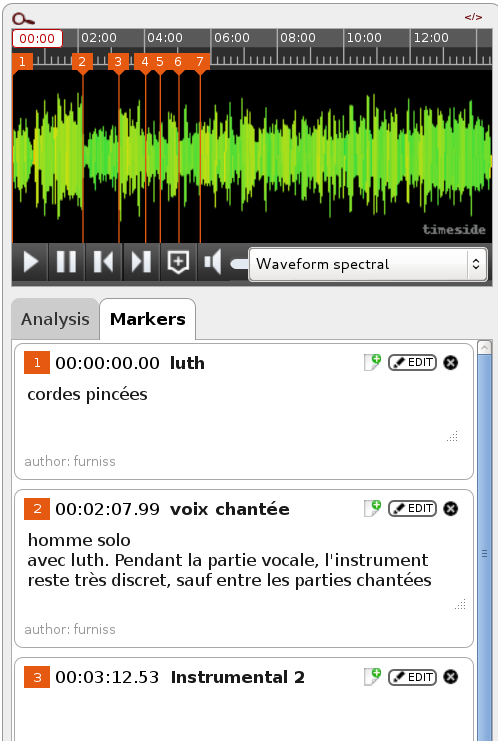
\includegraphics[width=\linewidth]{img/markers.png}
    \end{column}
  \end{columns}
\end{frame}

\section[TimeSide]{TimeSide, an audio analysis framework}\label{sec:TimeSide}
\subsection{Audio management}
\begin{frame}{TimeSide}\scriptsize
 \begin{block}{An open source web audio processing framework}
   \begin{itemize}
   \item TimeSide is the \alert{audio signal processing engine} of Telemeta developed and published as a separate project.
   \item \textbf{TimeSide = \textsf{web audio + signal processing + audio visualization + MIR}}  
   \item \alert{Python} and \alert{JavaScript}
   \end{itemize}
\vspace{-0.5cm}\begin{center}
  \colorbox{yellow!40}{\bf \url{https://github.com/parisson/TimeSide/} }
\end{center}
\end{block}
\begin{block}{Audio management}
  TimeSide provides the following main features:
  \begin{itemize}
   \item Smart dynamic audio player with enhanced visualization (e.g. waveform,
    spectrogram) that can be embedded into any html page through \emph{iframe} (live example: \href{http://yomix.org/telemeta-1-embedded-timeside-player.html}{Yomguy's blog})
  \item Multi-format support: decodes the vast majority of audio and
    video formats% through Gstreamer and transcodes them with smart
    %streaming and caching methods.
  \item On-the-fly audio analysis, transcoding, streaming and metadata embedding
    based on an easy plugin architecture.
  \end{itemize}
\end{block}

 
\end{frame} 

\begin{frame}{TimeSide engine architecture}
  \begin{figure}[htbp]
  \centering
  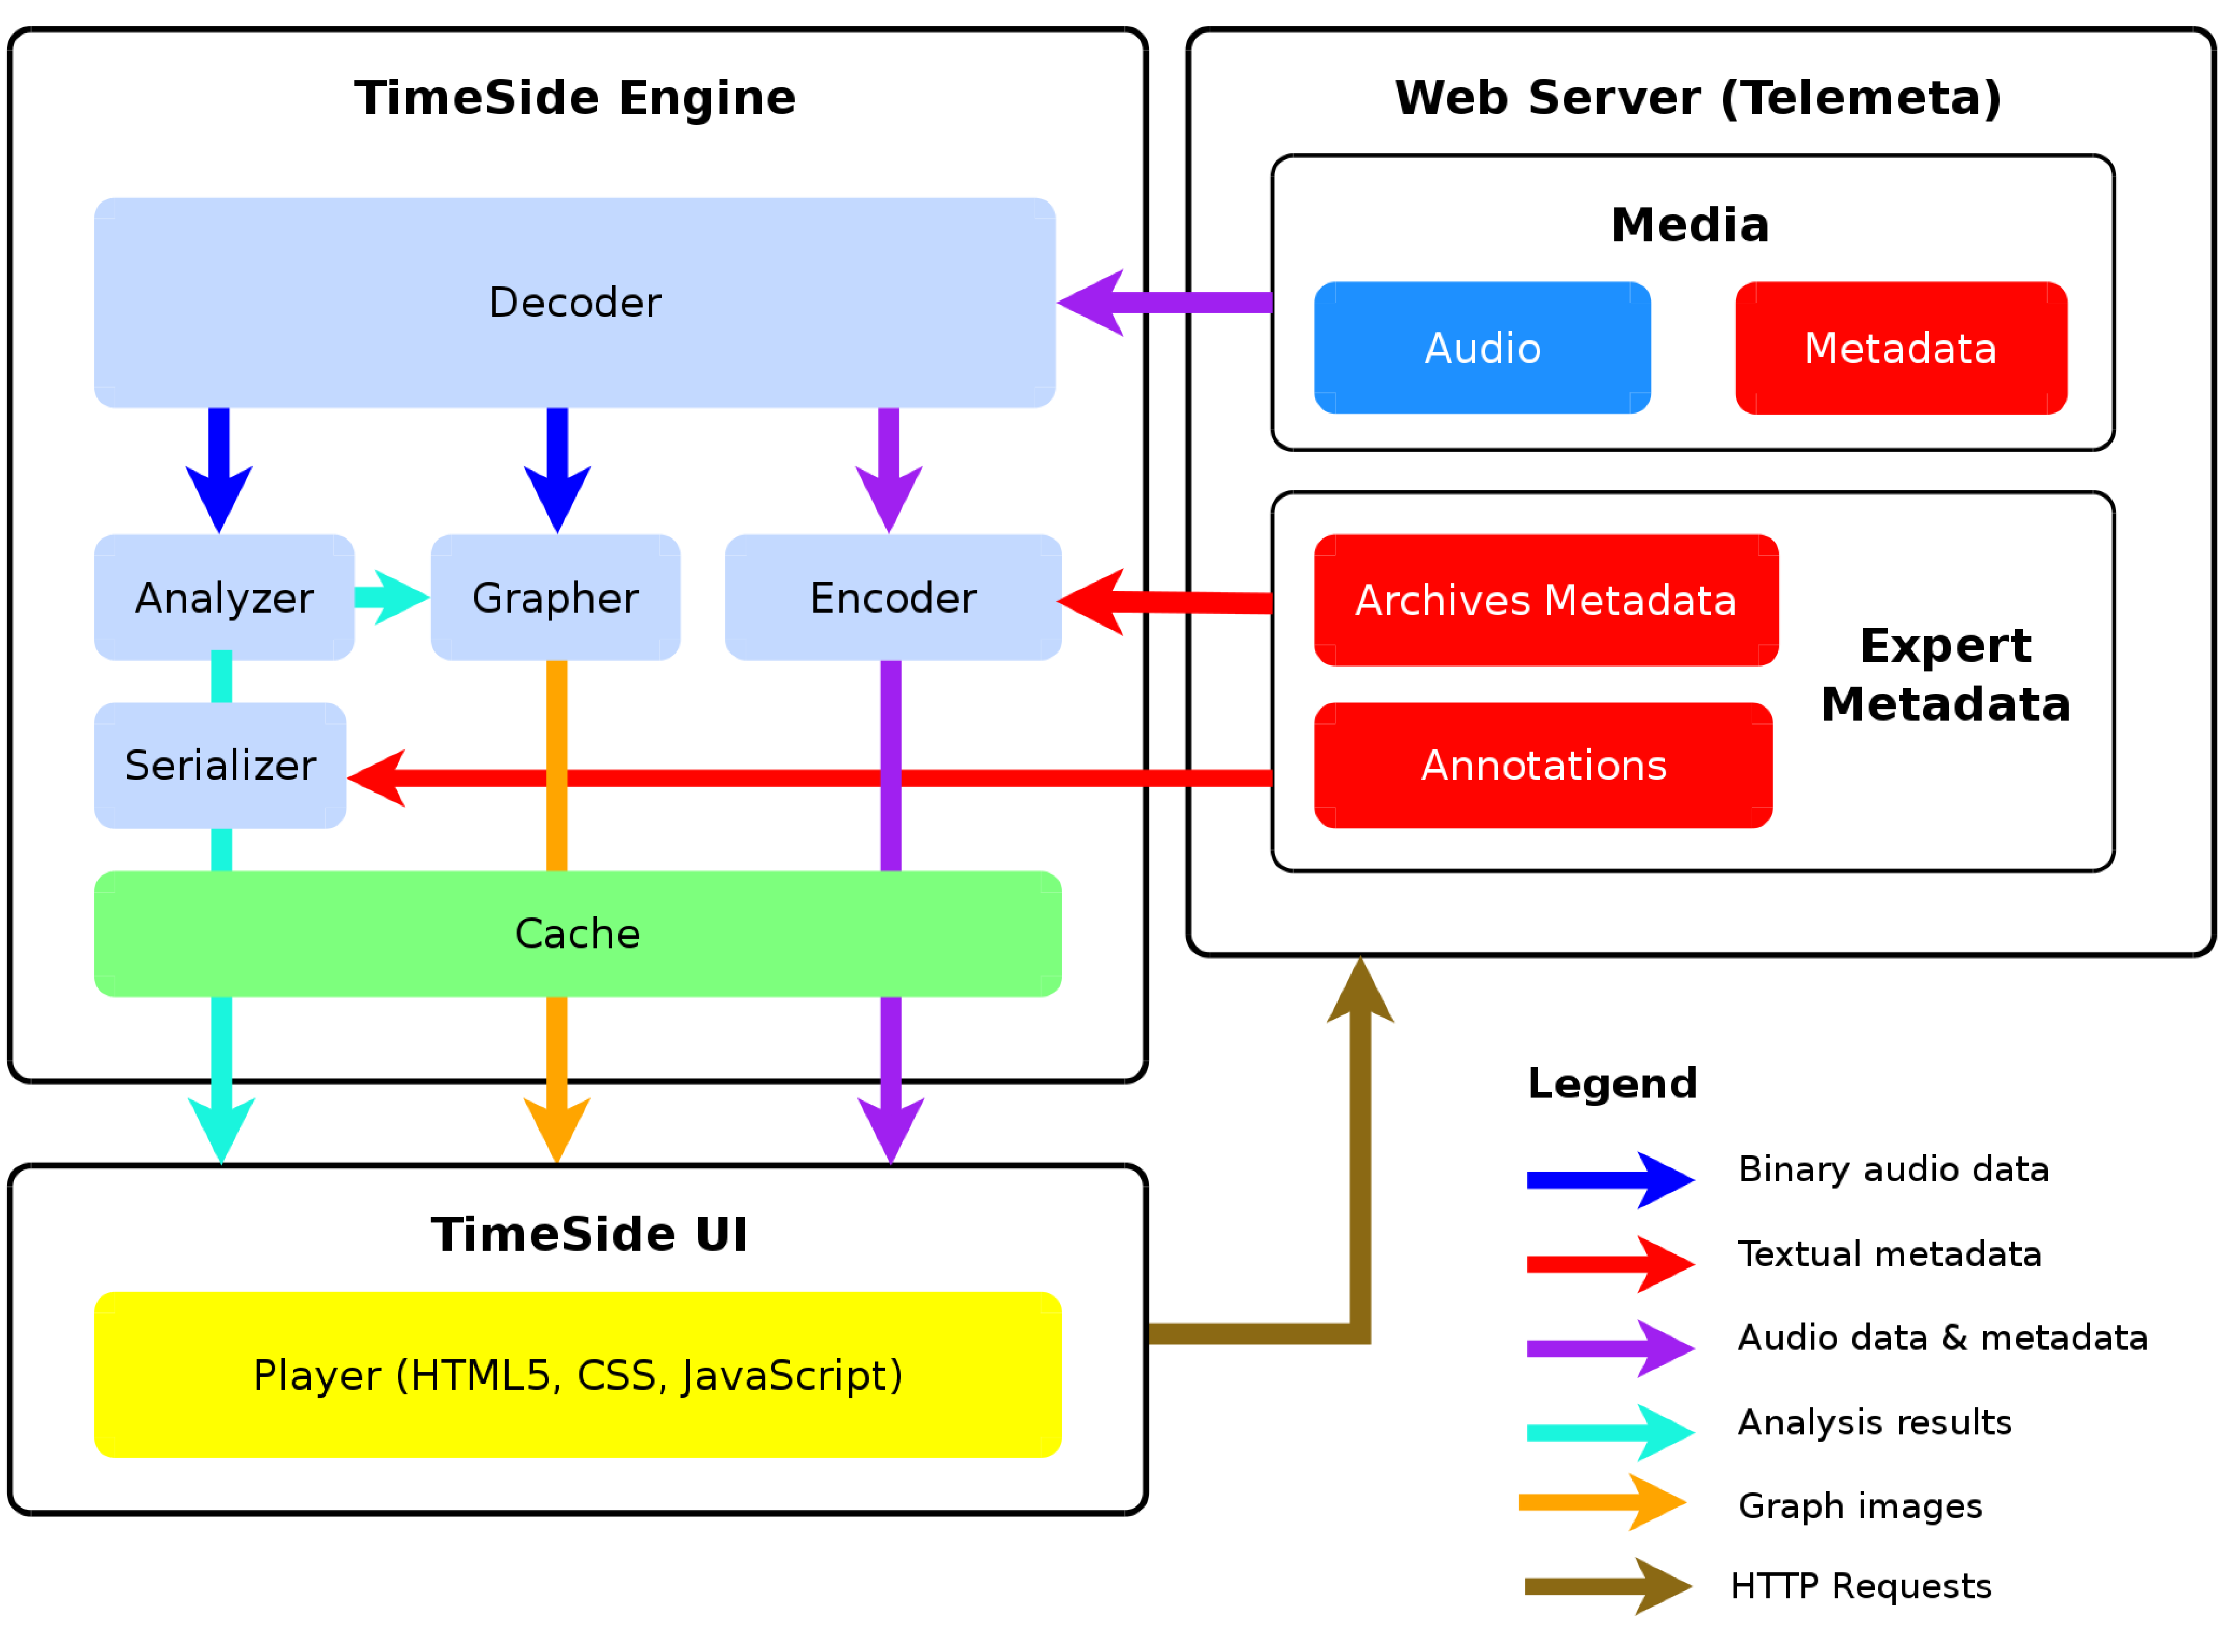
\includegraphics[width=0.8\linewidth]{img/timeside_schema_v3.pdf}
  \caption{TimeSide engine architecture and data flow with Telemeta web-server}\label{fig:TimeSide_Archi}
\end{figure}
\end{frame}
  
\begin{frame}
  \frametitle{TimeSide engine architecture}
  \begin{center}
    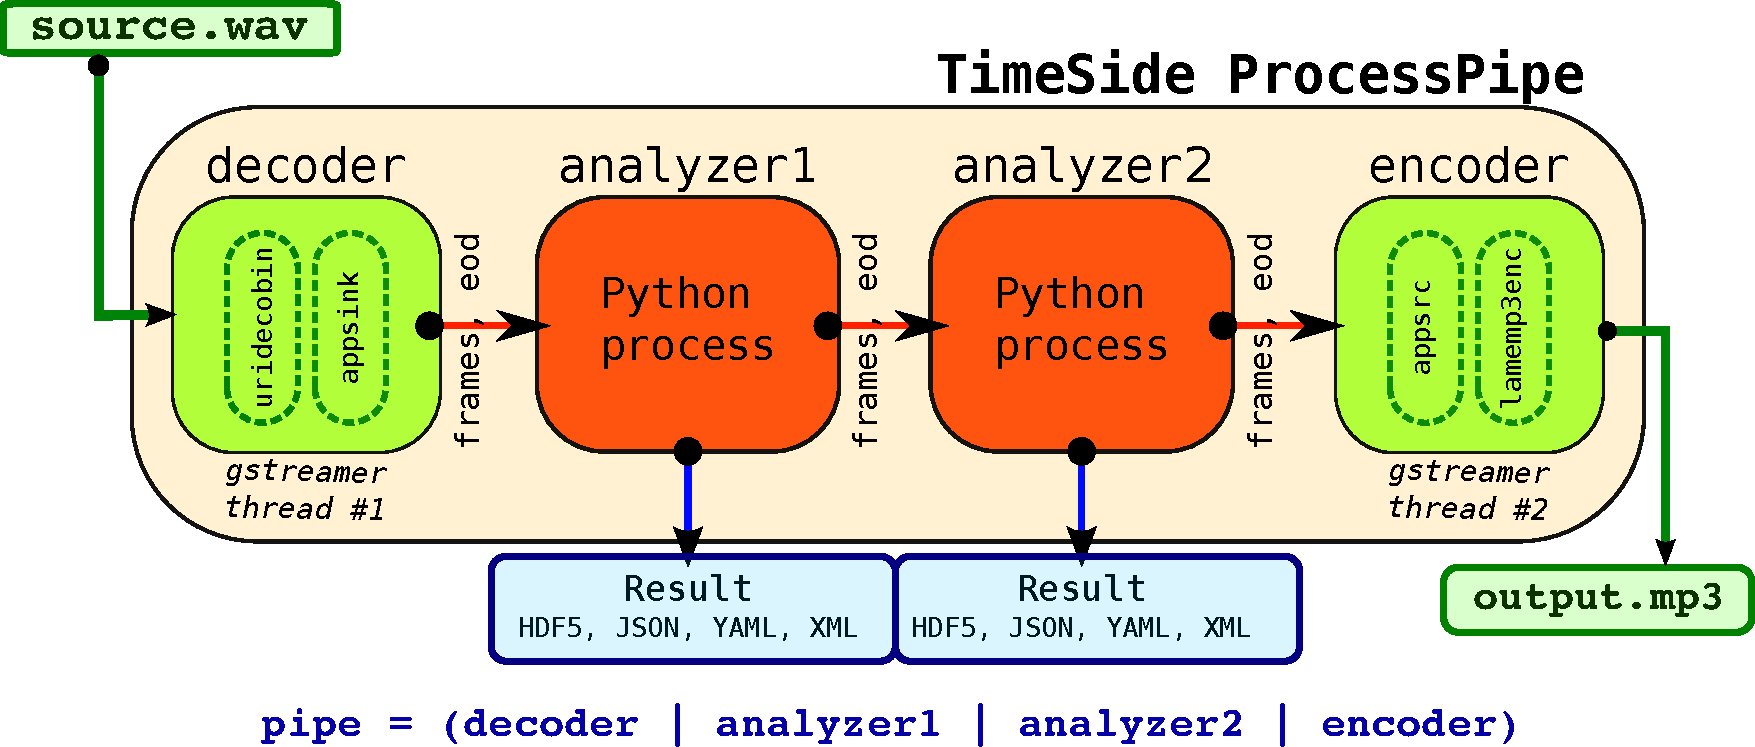
\includegraphics[width=0.95\textwidth]{img/TimeSide_pipe.pdf}
  \end{center}
  \begin{block}{Process Pipe}
    \begin{itemize}
    \item On-the-fly audio processing by simultaneous processors (decoder, encoders, analyzers, graphers)
    \item Use of \emph{Gstreamer} for audio decoding and encoding    \end{itemize}
  \end{block}
\end{frame}



\subsection{Audio features extraction}
\begin{frame}{Audio features extraction}
\begin{block}{Audio features extraction}
TimeSide incorporates some state-of-the-art \alert{audio feature extraction libraries} such as:
\vspace{-0.1cm}
\begin{itemize}
\item Aubio:
    \colorbox{yellow!30}{\scriptsize \url{http://aubio.org}}
\vspace{-0.1cm}
\item Yaafe:
    \colorbox{yellow!30}{\scriptsize \url{http://yaafe.sourceforge.net}}
\vspace{-0.1cm}
\item Vamp plugins:  
    \colorbox{yellow!30}{\scriptsize \url{http://www.vamp-plugins.org}}
\end{itemize}

Given the extracted features, every sound item in a given
  collection can be automatically analyzed.\\
The results of this
  analysis can be:
  \begin{itemize}\footnotesize
 \item Serialized to the web browser through common markup languages: JSON and YAML
  \item Stored in a scientific file format (e.g. \emph{NumPy} format or \emph{HDF5})
  \item Exported to sound visualization and annotation software
    (e.g. \emph{Sonic Visualizer, ELAN, transcriber})
 
  \end{itemize}
\end{block}

\end{frame}


\subsection{Analyzer Result Format}
\begin{frame}
  \frametitle{Analyzer Result (\emph{audio feature}) Format}
     \begin{block}{Result types: \\\emph{time mode} $\times$ \emph{data mode}}
       \begin{columns}
         \begin{column}{0.35\linewidth}
           \begin{itemize}
           \item Data modes:
             \begin{itemize}
             \item \alert<2-5>{Label}
             \item \alert<6-9>{Value}
             \end{itemize}
           \item Time modes:
             \begin{itemize}
             \item \alert<2,6>{Global}
             \item \alert<3,7>{Event}
             \item \alert<4,8>{Segment}
             \item \alert<5,9>{Framewise}
             \end{itemize}
           \end{itemize}
         \end{column}
         \begin{column}{0.50\linewidth}\footnotesize
           \begin{exampleblock}<2->{\footnotesize Result Container}\scriptsize
             \begin{itemize}
             \item ID Metadata
             \item Audio Metadata
             \item Parameters
             \item Data object
               \begin{itemize}\scriptsize
               \item<2-5> Label
               \item<2-5> Label Metadata ({\tiny label, label\_id, ...})
               \item<6-9> Value
               \item<3-4,7-8> Time
               \item<4,8> Duration
               \item<5,9> Frame Metadata ({\tiny sample rate, blocksize,
                 stepsize})
               \end{itemize}
           
             \end{itemize}
           \end{exampleblock}

         \end{column}
       \end{columns}
      
  \end{block}   
\end{frame}
\begin{frame}
\frametitle{Analyzer Result examples}
\begin{center}
  \includegraphics<1>[width=\linewidth]{img/results/IRIT_Speech4Hz.png}
  \includegraphics<2>[width=\linewidth]{img/results/SOLO_DUOdetection.png}\\
  {\footnotesize \only<1>{\url{http://diadems.telemeta.org/archives/items/CNRSMH_I_2013_201_001_01/}}
  \only<2>{\url{http://diadems.telemeta.org/archives/items/CNRSMH_I_2000_008_001_04/}}}
\end{center}
\end{frame}
\subsection{Ongoing developments}
\begin{frame}{Ongoing developments}
  \begin{block}{Data analysis for the web}
    \begin{itemize}
    \item New analyzers from Diadems project
    \item Advance data representations for the web: D3.js, WAVES.js (IRCAM)
    \item Zoom capabilities 
    \item Online computational tasks design and management
    \item REST Web-API is being developed to provide
audio analysis services over the web
    \end{itemize}
  \end{block}
    \begin{block}{Annotation functions: {\small time segments with free text and labels}}
      \begin{itemize}
      \item TimeSide: online annotation tool 
      \item Telemeta: collaborative annotation platform
      \item Virtuous circle between automatic analysis and annotations
      \end{itemize}
      
    \end{block}

  
\end{frame}
\section{Conclusion}
% \begin{frame}\frametitle{Conclusion}
%   The Telemeta open-source framework provides a new platform for researchers in humanities and social sciences to efficiently distribute, share and work on their research on musical and sound materials. 
% This platform offers automatic music analysis capabilities through the external component, TimeSide, which provides a flexible computational analysis engine together with web serialization and visualization options. 
% The Telemeta platform provides an appropriate processing framework for researchers in computational ethnomusicology to develop and evaluate their algorithms. 
% Deployed to manage the CNRS - Musée de l’Homme sound archives, the Telemeta platform has been conceived and adapted to generate tools in line with the needs of users. 

% Thanks to the collaborative nature of the platform, users can continuously enrich metadata associated with sound archives. 
% The benefits of this collaborative platform for the field of ethnomusicology apply to numerous aspects of research, ranging from musical analysis in diachronic and synchronic comparative perspectives, as well as the long-term preservation of sound archives and the support of teaching materials for education. 

% \end{frame}

\begin{frame}{Conclusion}
  \begin{block}{}
    \begin{itemize}[<+->]
    \item Telemeta is a \alert{fully operational} web audio framework
      for managing digital sound archives
    \item It's an \alert{open-source} software (-> feel free to use,
      fork or contribute)
    \item Through the Sound archives of the CNRS - Musée de l’Homme,
      it is now used by many ethnomusicologists around the world for
      research or education purposes.
    \item Its collaborative nature enable a \alert{continuous
        enrichment} of the audio content, the metadata and the
      analysis tools.
    \end{itemize}
  \end{block}
\end{frame}

\frame{\frametitle{Conclusion}
\begin{block}{Lessons learned from a 7 years old project}
\begin{itemize}
\item \alert{Simplicity} is better than complexity (\alert{KISS} principle)
\item \alert{Modularity} is only accessible with a flexible language (thanks Python!)
\item \alert{Models} and \alert{objects} are more important than technologies
\item A good \alert{workflow} is defined by the users themselves through \alert{feedback} and constant \alert{revisions}
\item \alert{Prototyping} and \alert{unit testing} are some crucial parts of the development process
\item A good platform relies on \alert{standards}, not on formats
\item The \alert{Open Source} ecosystem provides some tremendous possibilities to develop, deploy and scale a platform project
\end{itemize}
\end{block}
}


\begin{frame}{Conclusion}
  \begin{block}{Future developments}
Future developments will turn Telemeta into:
    \begin{itemize}
    \item an efficient \alert{annotation platform} (with zoom and segment selection)
    \item an \alert{social and collaborative platform} (user access managment and social stuff)
    \item an \alert{interdisciplinary} collaborative platform between IT and ethno with the joint develoment of automatic analysis and indexation tools
    \end{itemize}
  \end{block}
\end{frame}

\begin{frame}{The end}
 \begin{center}
   \large{Thank you!}\\
   \large{We are looking for new patners and projects,\\ let's keep in touch!}   
    \begin{block}{Links}
     \begin{itemize}\small
        \item \chref{http://telemeta.org}{telemeta.org}
        \item \chref{https://twitter.com/telemeta/}{@telemeta}
        \item \chref{http://github.com/Parisson/}{github.com/Parisson/}
    \end{itemize}
    \end{block}
    \begin{block}{Contact us}
    \begin{itemize}\small
    \item \chref{mailto:guillaume@parisson.com}{guillaume@parisson.com}, \chref{mailto:thomas@parisson.com}{thomas@parisson.com}
    \item \chref{https://twitter.com/yomguy/}{@yomguy}
    \item \chref{https://plus.google.com/u/0/+GuillaumePellerin/posts}{+GuillaumePellerin}
    \item \chref{http://fr.linkedin.com/in/guillaumepellerin}{fr.linkedin.com/in/guillaumepellerin}
    \end{itemize}
     \end{block}
  \end{center}
\end{frame}

\appendix
\section{Additional Materials}


    \begin{frame}{Sponsors}


        \begin{center}
        \begin{columns}[c]
        \column{2.5cm}
        \begin{center}
            \pgfimage[width=2cm]{img/logo-ANR}
        \end{center}
        \column{2.5cm}
        \begin{center}
            \pgfimage[width=1.5cm]{img/logo-CNRS-big}
        \end{center}
        \column{2.5cm}
        \begin{center}
            \pgfimage[width=2.5cm]{img/Logo_UPX_big}
        \end{center}
        \column{2cm}
        \begin{center}
            \pgfimage[width=2cm]{img/upmc}
        \end{center}
        \end{columns}
        \end{center}

        \begin{center}
        \begin{columns}[c]
        \column{2.5cm}
        \begin{center}
            \pgfimage[width=1.5cm]{img/logo_mcc_3}
        \end{center}
        \column{2.5cm}
        \begin{center}
            \pgfimage[width=1.5cm]{img/logo-MNHN-big}
        \end{center}
        \column{2.5cm}
        \begin{center}
            \pgfimage[width=1.5cm]{img/logohumanum-web-grand-rvb}
        \end{center}
        \column{2cm}
        \begin{center}
            \pgfimage[width=2.5cm]{img/parisson_logo_200}
        \end{center}
        \end{columns}
        \end{center}

        
        \begin{center}
            \pgfimage[width=4.5cm]{img/europeana-sounds_0}
        \end{center}
        
    \end{frame}
    
    
\subsubsection{Telemeta - Geographic Navigator}
\begin{frame}[plain, label=geonavigator]{Telemeta - Geographic Navigator}
  \begin{center}
    \fbox{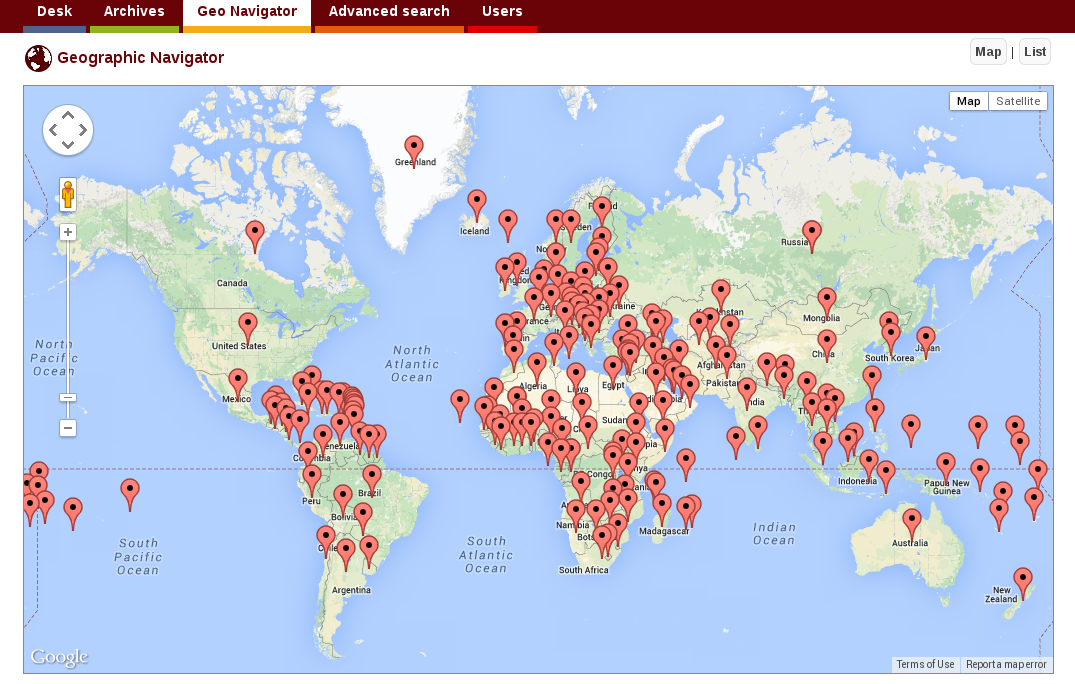
\includegraphics[width=\linewidth]{img/telemeta_geo.png}}
  \end{center}
\hyperlink{telemeta_features}{\beamerbutton{back}}
\end{frame}
\subsubsection{Multi language support}
\begin{frame}[label=telemeta_languages]{Telemeta - Multi language support}
\only<1>{\framesubtitle{English}}
\only<2>{\framesubtitle{French}}
\only<3>{\framesubtitle{German}}
\only<4>{\framesubtitle{Chinese}}
\only<5>{\framesubtitle{Arabic}}
\only<5>{\framesubtitle{Portuguese}}

  \begin{center}
    \includegraphics<1>[width=1.1\textwidth]{img/telemeta_english.png}
    \includegraphics<2>[width=1.1\textwidth]{img/telemeta_french.png}
    \includegraphics<3>[width=1.1\textwidth]{img/telemeta_german.png}
    \includegraphics<4>[width=1.1\textwidth]{img/telemeta_chinese.png}
    \includegraphics<5>[width=1.1\textwidth]{img/telemeta_arabic.png}
    \includegraphics<6>[width=1.1\textwidth]{img/telemeta_portuguese.png}

  \end{center}
\hyperlink{telemeta_features}{\beamerbutton{back}}
\end{frame}
\subsubsection{Metadata}
\begin{frame}[label=metadata_example]{Contextual Information example: Collection}
  \begin{center}
    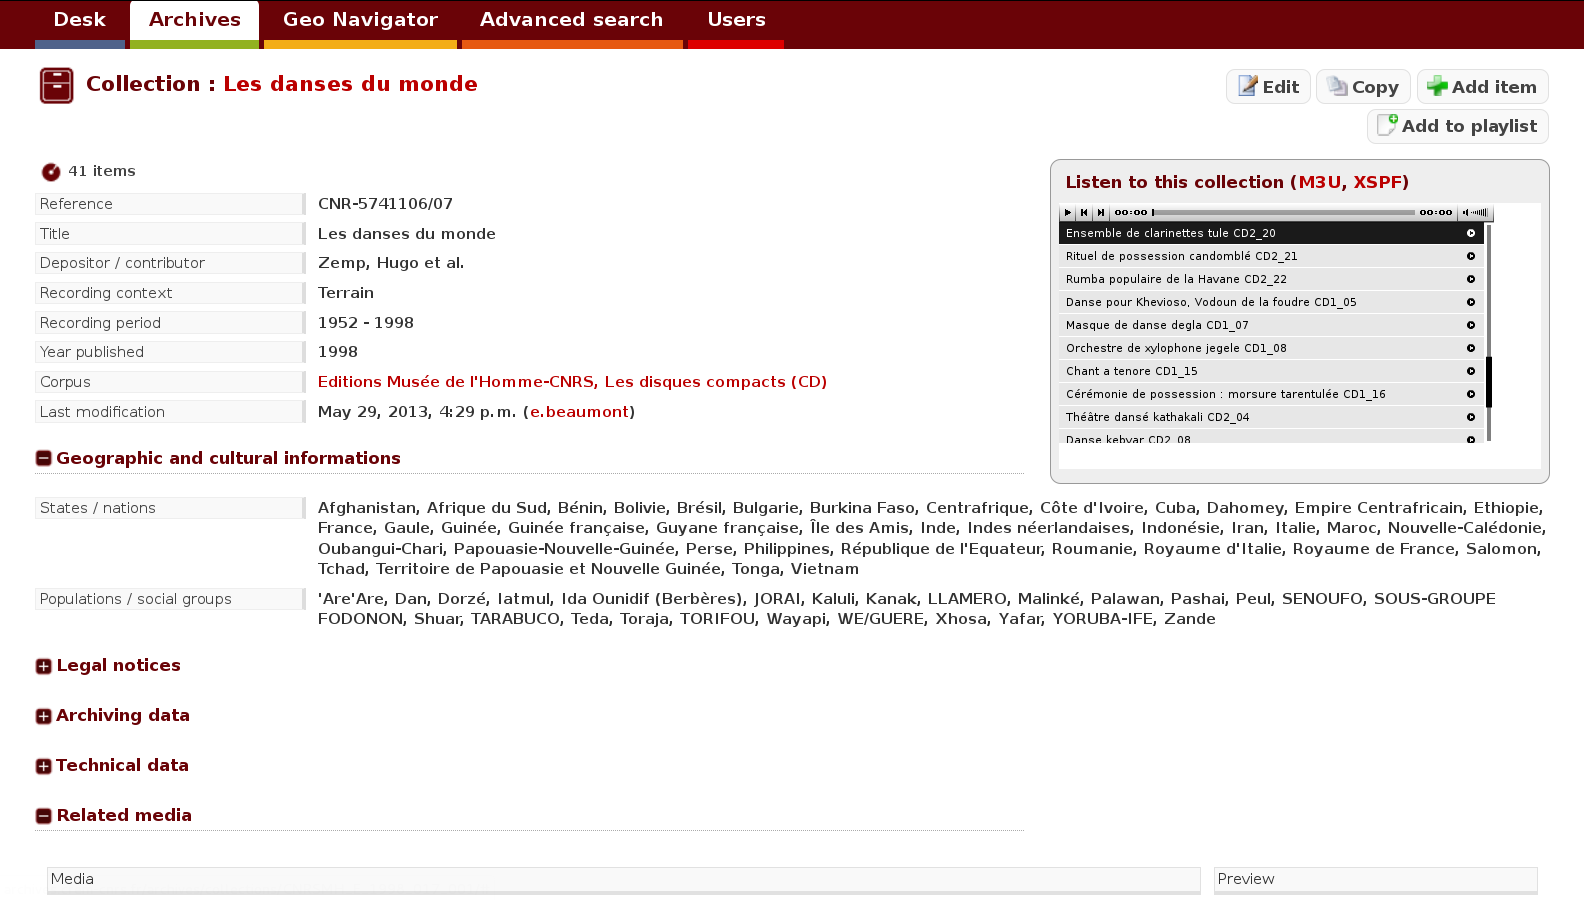
\includegraphics[width=1\textwidth]{img/telemeta_metadata_collection.png}
  \end{center}
\href{http://archives.crem-cnrs.fr/archives/collections/CNRSMH_E_1998_017_001/}{\beamerbutton{Online}}
 \href{./captures/Collection.html}{\beamerbutton{Offline}}
\hyperlink{telemeta_metadata}{\beamerbutton{back}}
\end{frame}
\begin{frame}{Contextual Information example: Item}
  \begin{center}
    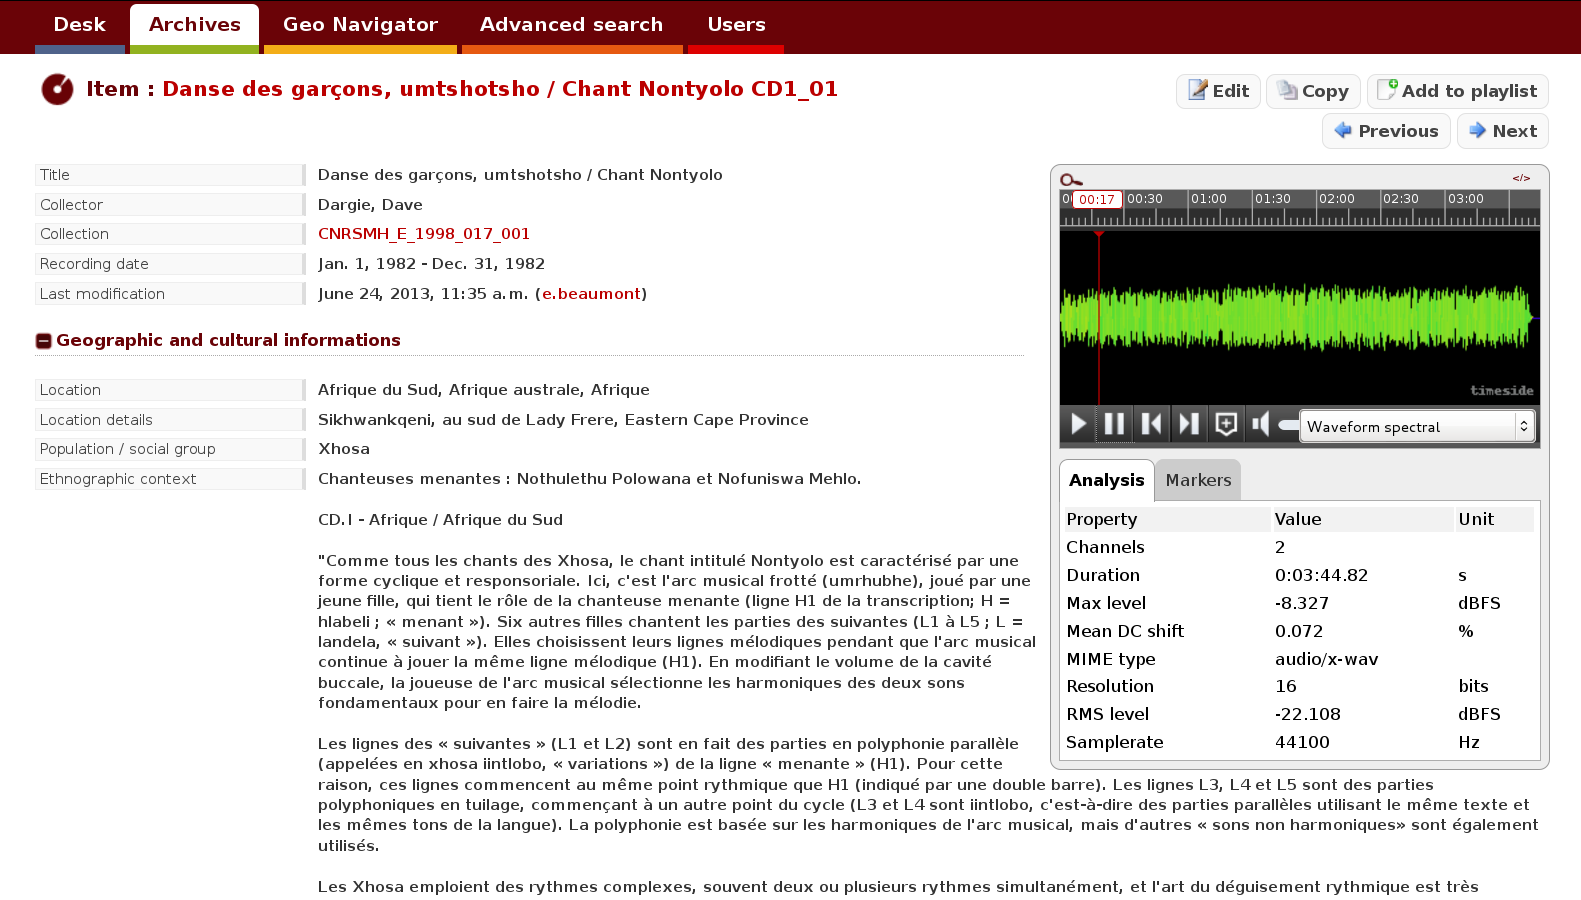
\includegraphics[width=1\textwidth]{img/telemeta_metadata_item.png}
  \end{center}
  \href{http://archives.crem-cnrs.fr/archives/items/CNRSMH_E_1998_017_001_001_01/}{\beamerbutton{Online}}
 \href{./captures/Item.html}{\beamerbutton{Offline}}
\hyperlink{telemeta_metadata}{\beamerbutton{back}}
\end{frame}

%%% Local Variables: 
%%% mode: latex
%%% TeX-master: t
%%% End: 
\end{document}